\section{Graph-Derived Architecture Reference}
\label{app:graph}

The monorepo maintains a machine-readable architecture graph in \texttt{graph-metadata.json}, regenerated via \texttt{bun run graph}. Figure~\ref{fig:graph-overview} visualizes the five logical communities; Tables~\ref{tab:graph-dataflows} and~\ref{tab:graph-communities} list selected data-flow edges and cluster definitions extracted from the same source.

\begin{figure}[t]
  \centering
  \IfFileExists{figures/graph-overview.pdf}{%
    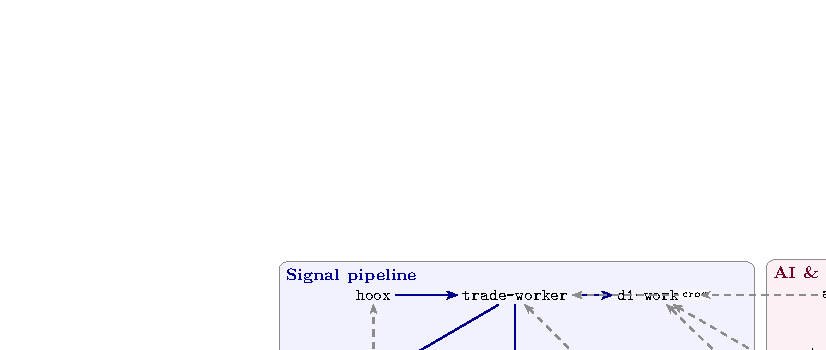
\includegraphics[width=0.98\linewidth]{figures/graph-overview.pdf}%
  }{%
    \ifhooxusetikz
      \resizebox{0.98\linewidth}{!}{% TikZ: code-graph community clusters (from graph-metadata.json)
% Layout:
%   - top-left: Signal pipeline cluster (hoox, trade-worker, d1-worker top row;
%               telegram-worker, analytics-worker bottom row)
%   - top-right: AI & risk cluster (agent-worker + telegram-worker/RAG)
%   - bottom-left: Packages cluster (hoox-shared, hoox CLI)
%   - bottom-right: Ingress & ops cluster (email-worker, report-worker, dashboard)
\begin{tikzpicture}[
  x=1cm, y=1cm,
  cluster/.style={draw=black!45, rounded corners=4pt, inner sep=0.40cm},
  clabel/.style={font=\footnotesize\bfseries, anchor=north west},
  worker/.style={font=\footnotesize\ttfamily, align=center, inner sep=2pt},
  infra/.style={font=\scriptsize\ttfamily, align=center, text=black!65, inner sep=2pt},
  flow/.style={-{Stealth[length=1.8mm]}, semithick, draw=blue!55!black},
  auxflow/.style={-{Stealth[length=1.5mm]}, semithick, dashed, draw=black!45}
]

  % ── Signal pipeline cluster (top-left) ──
  % 2.4cm horizontal spacing so worker labels don't collide
  \node[worker] (hoox) at (0.0, 0.0)  {hoox};
  \node[worker] (tw)   at (2.4, 0.0)  {trade-worker};
  \node[worker] (d1)   at (4.8, 0.0)  {d1-worker};
  \node[worker] (tg)   at (0.0,-1.4)  {telegram-worker};
  \node[worker] (anw)  at (2.4,-1.4)  {analytics-worker};
  \node[infra]  (spinfra) at (4.8,-1.4) {Queue, Idempotency\\DO, D1};

  \begin{scope}[on background layer]
    \node[cluster, fit=(hoox)(tw)(d1)(tg)(anw)(spinfra),
      fill=blue!5, label={[clabel, text=blue!60!black]north west:Signal pipeline}] (spbox) {};
  \end{scope}

  \draw[flow] (hoox) -- (tw);
  \draw[flow] (tw)   -- (d1);
  \draw[flow] (tw)   -- (tg);
  \draw[flow] (tw)   -- (anw);

  % ── AI & risk cluster (top-right) ──
  \node[worker] (aw)     at (8.5, 0.0)  {agent-worker};
  \node[worker] (tgrag)  at (8.5,-1.0)  {telegram-worker};
  \node[infra]  (aiinfra) at (8.5,-1.85) {Workers AI, Vectorize};

  \begin{scope}[on background layer]
    \node[cluster, fit=(aw)(tgrag)(aiinfra),
      fill=purple!6, label={[clabel, text=purple!60!black]north west:AI \& risk}] (aibox) {};
  \end{scope}

  \draw[auxflow] (aw) -- node[font=\tiny, fill=white, inner sep=1pt] {cron} (tw);
  \draw[auxflow] (aw) -- (d1);

  % ── Shared packages (bottom-left) ──
  \node[worker] (shared) at (0.0, -3.6) {hoox-shared};
  \node[worker] (cli)    at (2.4, -3.6) {hoox CLI};
  \begin{scope}[on background layer]
    \node[cluster, fit=(shared)(cli),
      fill=green!6, label={[clabel, text=green!50!black]north west:Packages}] (pkgbox) {};
  \end{scope}

  % ── Infrastructure + auxiliary workers (bottom-right) ──
  \node[worker] (email)  at (6.0, -3.6) {email-worker};
  \node[worker] (report) at (8.5, -3.6) {report-worker};
  \node[worker] (dash)   at (11.0,-3.6) {dashboard};
  \node[infra]  (infrow) at (8.5,-4.5)  {R2, KV, Browser\\Rendering, Analytics Engine};
  \begin{scope}[on background layer]
    \node[cluster, fit=(email)(report)(dash)(infrow),
      fill=orange!6, label={[clabel, text=orange!60!black]north west:Ingress \& ops}] (opsbox) {};
  \end{scope}

  \draw[auxflow] (email) -- (tw);
  \draw[auxflow] (report) -- (d1);
  \draw[auxflow] (dash) -- (d1);

  \draw[auxflow] (shared.north) -- ++(0,0.5) -| (hoox.south);
  \draw[auxflow] (shared.north) -- ++(0,0.5) -| (aw.south);

\end{tikzpicture}
}%
    \else
      \fbox{\parbox{0.92\linewidth}{\small Signal pipeline, AI/risk, packages, and ingress/ops clusters from \texttt{graph-metadata.json}}}
    \fi
  }
  \caption{Code-graph community overview. Solid arrows: primary signal path; dashed arrows: cron, shared-library, or auxiliary ingress.}
  \label{fig:graph-overview}
\end{figure}

\IfFileExists{generated/graph-tables.tex}{%
  % Auto-generated by papers/scripts/sync-graph-tables.ts — do not edit by hand.
% Generated: 2026-07-11T08:43:14.977Z
% Included from appendices/E-graph-reference.tex (section header lives there).

\subsection{Data-flow edges}

\begin{table}[h]
\centering
\caption{Primary data-flow edges (selected).}
\label{tab:graph-dataflows}
\small
\begin{tabular}{@{}llp{6.8cm}@{}}
\toprule
\textbf{Source} & \textbf{Target} & \textbf{Description} \\
\midrule
\texttt{hoox} & \texttt{trade-worker} & Trading signal: POST /webhook → validate webhook + check kill\_switch + check IP allowlist + deduplicate via IdempotencyStore DO + check rate limit → produce TradeQueueMessage to TRADE\_QUEUE → trade-worker consumes from queue handler with exponential backoff retry (max 5) \\
\texttt{trade-worker} & \texttt{d1-worker} & Trade data persistence: executeTrade → on success, write trade record + update positions + log to system\_logs via d1-worker POST /query (INSERT/UPDATE) with X-Internal-Auth-Key. Reported via DbLogger request/response log pairs. \\
\texttt{trade-worker} & \texttt{telegram-worker} & Trade notification: executeTrade → on success or failure, call telegram-worker POST /process (legacy) or POST /webhook with NotificationPayload \{ message, chatId? \} via TELEGRAM\_SERVICE service binding \\
\texttt{trade-worker} & \texttt{analytics-worker} & Trade analytics: executeTrade → trackAnalytics(env, '/track/api-call', \{ worker: 'trade-worker', endpoint, latencyMs, success \}) for every /webhook and /process call. Fire-and-forget via ctx.waitUntil. \\
\texttt{agent-worker} & \texttt{d1-worker} & Position monitoring: runHousekeeping → reads open positions from D1 via D1\_SERVICE binding (POST /query: SELECT * FROM positions WHERE status = 'OPEN'). Checks trailing stops from CONFIG\_KV (prefix: trade:watermark:). \\
\texttt{agent-worker} & \texttt{trade-worker} & Risk adjustment: processRoutine → AI risk assessment → if adjustment needed, calls trade-worker POST /webhook via TRADE\_SERVICE binding with X-Internal-Auth-Key. Close orders via sendCloseOrder. \\
\texttt{agent-worker} & \texttt{telegram-worker} & Risk alert: runHousekeeping/processRoutine → on risk threshold breach or trailing stop triggered, calls telegram-worker POST /webhook with alert message via TELEGRAM\_SERVICE binding. Fire-and-forget. \\
\texttt{email-worker} & \texttt{trade-worker} & Email signal: Mailgun webhook POST /webhook → HMAC-SHA256 signature validation → parseEmailSignal (JSON or plaintext regex extraction) → forward parsed EmailSignal to trade-worker POST /webhook via TRADE\_SERVICE binding with X-Internal-Auth-Key header \\
\texttt{email-worker} & \texttt{analytics-worker} & Email analytics: on signal forward (success or failure), trackAnalytics(env, '/track/signal', \{ source: 'email-worker', type, symbol, confidence \}). Fire-and-forget via ctx.waitUntil. \\
\texttt{d1-worker} & \texttt{analytics-worker} & DB analytics: on every POST /query and POST /batch execution, trackAnalytics(env, '/track/api-call', \{ worker: 'd1-worker', endpoint, latencyMs, success \}). Fire-and-forget via ctx.waitUntil. \\
\texttt{telegram-worker} & \texttt{analytics-worker} & Notification analytics: after each notification send, trackAnalytics via internal function call (not service binding). Tracks notification type, target, and success status. \\
\texttt{web3-wallet-worker} & \texttt{telegram-worker} & Web3 notification: on wallet initialization, calls telegram-worker POST /webhook with wallet address notification via TELEGRAM\_SERVICE service binding. Fire-and-forget via ctx.waitUntil. \\
\texttt{web3-wallet-worker} & \texttt{analytics-worker} & Web3 analytics: after wallet init, trackAnalytics(env, '/track/api-call', \{ worker: 'web3-wallet-worker', endpoint: '/', latencyMs, success \}). Fire-and-forget via ctx.waitUntil. \\
\texttt{report-worker} & \texttt{telegram-worker} & Report delivery: generateAndStoreReport → on PDF stored in R2, calls telegram-worker POST /process via TELEGRAM\_SERVICE binding with markdown message including signed report URL. Fire-and-forget via ctx.waitUntil. \\
\texttt{dashboard} & \texttt{d1-worker} & Dashboard data read: Next.js server components call d1-worker service binding (GET /api/balances, GET /api/positions, GET /api/settings, GET /api/logs, POST /query) for dashboard page rendering and API routes. Passes X-Internal-Auth-Key via env.D1\_SERVICE binding. \\
\texttt{dashboard} & \texttt{agent-worker} & Dashboard status: dashboard calls agent-worker POST /agent/housekeeping via AGENT\_SERVICE binding to trigger on-demand AI risk assessment and display results on dashboard status page. \\
\bottomrule
\end{tabular}
\end{table}

\subsection{Architecture communities}

\begin{table}[h]
\centering
\caption{Logical node clusters in the code graph.}
\label{tab:graph-communities}
\small
\begin{tabular}{@{}llp{7.5cm}@{}}
\toprule
\textbf{ID} & \textbf{Label} & \textbf{Description} \\
\midrule
\texttt{workers} & Cloudflare Workers & All 10 worker services in the Hoox trading system \\
\texttt{packages} & Shared Packages & Reusable packages shared across workers \\
\texttt{infrastructure} & Cloudflare Infrastructure & D1, R2, KV, Queue, DO, AI, Vectorize, Analytics Engine, Browser Rendering \\
\texttt{signal-pipeline} & Signal Processing Pipeline & The core trading signal flow: hoox receives webhooks → deduplicate via IdempotencyStore DO → produce to TRADE\_QUEUE → trade-worker consumes with retry → execute on Binance/MEXC/Bybit → persist to D1 → notify via telegram → track via analytics-worker. Includes infrastructure nodes that enable this flow (queue, DO, D1 database). \\
\texttt{ai-system} & AI \& Risk Management & Autonomous AI risk management subsystem: agent-worker (5-min cron) reads positions from D1, assesses risk via Workers AI (with multi-provider fallback: workers-ai → openai → anthropic → google), adjusts positions via trade-worker, sends alerts via telegram-worker. Uses Vectorize index for RAG context retrieval. Embeddings generated via Workers AI. \\
\bottomrule
\end{tabular}
\end{table}

%
}{%
  \paragraph{Graph tables unavailable.} Run \texttt{make graph-tables} from the \texttt{papers/} directory to generate data-flow and community tables from \texttt{graph-metadata.json}.
}